\documentclass[a4paper]{article}

\usepackage[english]{babel}
\usepackage[utf8]{inputenc}
\usepackage{csquotes}
\usepackage{amsmath, latexsym}
\usepackage{graphicx}
\usepackage{tikz}
\usepackage{listings}
\usepackage{verbatim}
\usepackage{bigints}
\usepackage{float}
\usepackage{titling}
\usepackage[percent]{overpic}
\usepackage[para]{footmisc}
\usepackage[colorinlistoftodos]{todonotes}
\usepackage[style=authoryear,sorting=nty,maxcitenames=1]{biblatex}

\title{Spherically symmetric bubble collapse problem}
\author{}
\date{\today}

\begin{document}
\maketitle
\section*{Objective}
The present work aims to compute the suitable distance to place the Kirchhoff control surface from the bubble center where the linear acoustic wave equation is valid. For this, we solve the bubble collapse problem in one dimension, assuming spherical symmetry, and obtain the distance at which the ratio of acoustic pressure and ambient pressure of the fluid $p'/p_0 << 1$.  
\section*{Governing equation}
The Compressible Euler equations assuming spherical symmetry for the mulitphase system can be written as
\begin{align}
    (\rho)_t + (\rho u)_r &= \frac{-2\rho u}{r},\\
    (\rho u)_t + (\rho u^2 + p)_r &= \frac{-2\rho u^2}{r}, \\
    (E)_t + ((E + p) u)_r &= \frac{-2(E + p) u}{r},\\
    (\phi)_t + (\phi u)_r &= \phi u_r,
\end{align}
where the equation of state for the mixture is given by 
\begin{align}
    p &= (\gamma - 1)(E - \rho u^2/2) - \gamma P^{\infty},\\    
    \gamma &= 1 + \frac{(\gamma_w - 1)(\gamma_a - 1)}{(1 - \phi)(\gamma_w - 1) + \phi(\gamma_a  - 1)},\\
    P^{\infty} &= \frac{\gamma - 1}{\gamma}\Big( \phi \frac{\gamma_w P^\infty_w}{\gamma_w - 1}  +(1 - \phi)\frac{\gamma_a P^\infty_a}{\gamma_a - 1} \Big). 
\end{align}
\subsection*{Initial condition}
An air bubble of radius $R$ is placed in a water medium, assuming the fluid to be stationary. The initial condition for the primitive variables is given by
\begin{align}
    \rho &= \frac{(\rho_a + \rho_w)}{2} + \frac{(\rho_w - \rho_a)}{2}{\tanh\Big(\frac{r - R}{\epsilon h}}\Big),\\
    u &= 0,\\
    p &= \frac{(p_a + p_w)}{2} + \frac{(p_w - p_a)}{2}{\tanh\Big(\frac{r - R}{\epsilon h}}\Big),\\    
    \phi &= \frac{(\phi_a + \phi_w)}{2} + \frac{(\phi_w - \phi_a)}{2}{\tanh\Big(\frac{r - R}{\epsilon h}}\Big).
\end{align}

\begin{figure}[!h]
\centering
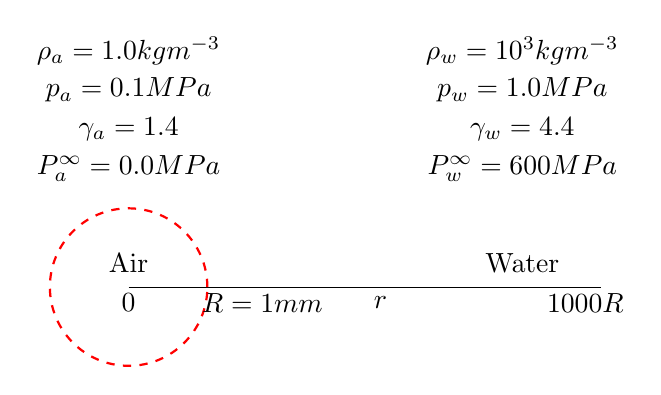
\begin{tikzpicture}
    \draw (0, 0) -- (6.0,0);
    \draw [red, thick, dashed] (0, 0) circle (1);
    \draw (1.7, -0.2) node {$R = 1mm$};
    \draw (3.2, -0.2) node {$r$};
    \draw (5.8, -0.2) node {$1000R$};
    \draw (0.0, 0.3) node {Air};
    \draw (5.0, 0.3) node {Water};
    \draw (0.0, -0.2) node {0};
    \draw (0.0, 3.0) node {$\rho_a = 1.0 kgm^{-3}$};
    \draw (0.0, 2.5) node {$p_a = 0.1 MPa$};
    \draw (0.0, 2.0) node {$\gamma_a = 1.4$};
    \draw (0.0, 1.5) node {$P^{\infty}_a = 0.0 MPa$};

    \draw (5.0, 3.0) node {$\rho_w = 10^3 kgm^{-3}$};
    \draw (5.0, 2.5) node {$p_w = 1.0 MPa$};
    \draw (5.0, 2.0) node {$\gamma_w = 4.4$};
    \draw (5.0, 1.5) node {$P^{\infty}_w = 600 MPa$};
\end{tikzpicture}
\caption{Schematic of air bubble in water medium with the initial conditions.}
\end{figure}

\subsection*{Boundary condition}
We enforce homogeneous Neumann boundary condition at both ends of the domain $\frac{\partial(*)}{\partial r}\Big |_0 = \frac{\partial(*)}{\partial r}\Big |_L = 0$.

\subsection*{Scaling}
Let $\bar{p}$ be the pressure scale, $\bar{\rho}$ be the density scale and $\bar{x}$ be the length scale. Then
\begin{equation}
    p = \bar{p}p_s, \;\;\;\; \rho = \bar{\rho} \rho_s, \;\;\;\; x = \bar{l}x_s. 
\end{equation}
Where $p_s, \rho_s$ and $x_s$ are the scaled pressure, density and length. We can obtain the velocity and time scale from the above scales.
\begin{equation}
    \frac{M}{LT^2} = \bar{p}\frac{M_s}{L_sT^2_s}, \;\;\;\; \frac{M}{L^3} = \bar{\rho}\frac{M_s}{L^3_s}.
\end{equation}
From the above relations we can obtain,
\begin{equation}
    \frac{L}{T} = \sqrt{\frac{\bar{p}}{\bar{\rho}}}\frac{L_s}{T_s}
\end{equation}
Therefore the velocity and time scale is given by
\begin{equation}
    v = \sqrt{\frac{\bar{p}}{\bar{\rho}}} v_s, \;\;\;\; t = \bar{l} \sqrt{\frac{\bar{\rho}}{\bar{p}}} t_s. 
\end{equation}
For the bubble problem we use the following scales,
\begin{equation}
    \bar{p} = 10^6Pa, \;\;\;\; \bar{\rho} = 1000 kgm^{-3}, \;\;\;\; \bar{l} = 10^{-3} m.
\end{equation}
The scaled initial conditions are
\begin{figure}[!h]
    \centering
    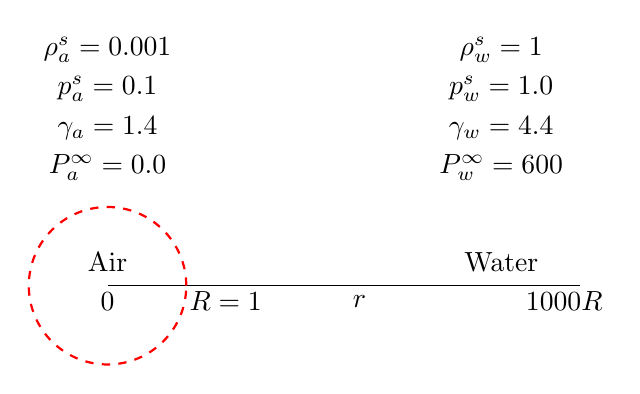
\begin{tikzpicture}
        \draw (0, 0) -- (6.0,0);
        \draw [red, thick, dashed] (0, 0) circle (1);
        \draw (1.5, -0.2) node {$R = 1$};
        \draw (3.2, -0.2) node {$r$};
        \draw (5.8, -0.2) node {$1000R$};
        \draw (0.0, 0.3) node {Air};
        \draw (5.0, 0.3) node {Water};
        \draw (0.0, -0.2) node {0};
        \draw (0.0, 3.0) node {$\rho_a^s = 0.001$};
        \draw (0.0, 2.5) node {$p_a^s = 0.1 $};
        \draw (0.0, 2.0) node {$\gamma_a = 1.4$};
        \draw (0.0, 1.5) node {$P^{\infty}_a = 0.0$};
    
        \draw (5.0, 3.0) node {$\rho_w^s = 1$};
        \draw (5.0, 2.5) node {$p_w^s = 1.0 $};
        \draw (5.0, 2.0) node {$\gamma_w = 4.4$};
        \draw (5.0, 1.5) node {$P^{\infty}_w = 600 $};
    \end{tikzpicture}
    \caption{Schematic of air bubble in water medium with the initial conditions.}
    \end{figure}

\end{document}
